%% Template pour rapport de stage du master AIC (Apprentissage,
%% Information et Contenu), Universit� Paris-Saclay
%% Template d'origine :
%% Copyright (C) 2008 Johan Oudinet <oudinet@lri.fr>
%%
%% Permission is granted to make and distribute verbatim copies of
%% this manual provided the copyright notice and this permission notice
%% are preserved on all copies.
%%
%% Permission is granted to process this file through TeX and print the
%% results, provided the printed document carries copying permission
%% notice identical to this one except for the removal of this paragraph
%% (this paragraph not being relevant to the printed manual).
%%
%% Permission is granted to copy and distribute modified versions of this
%% manual under the conditions for verbatim copying, provided that the
%% entire resulting derived work is distributed under the terms of a
%% permission notice identical to this one.
%%
%% Permission is granted to copy and distribute translations of this manual
%% into another language, under the above conditions for modified versions,
%% except that this permission notice may be stated in a translation
%% approved by the Free Software Foundation
%%

\documentclass[oneside]{memoir}
\let\STARTCODE\relax 
\let\STOPCODE\relax 
\STARTCODE
\usepackage{color,calc,graphicx,soul}
\definecolor{nicered}{rgb}{.647,.129,.149} \makeatletter
\newlength\dlf@normtxtw \setlength\dlf@normtxtw{\textwidth}
\def\myhelvetfont{\def\sfdefault{mdput}} \newsavebox{\feline@chapter}
\newcommand\feline@chapter@marker[1][4cm]{%
  \sbox\feline@chapter{%
    \resizebox{!}{#1}{\fboxsep=1pt%
      \colorbox{nicered}{\color{white}\bfseries\sffamily\thechapter}%
    }}%
  \rotatebox{90}{%
    \resizebox{%
      \heightof{\usebox{\feline@chapter}}+\depthof{\usebox{\feline@chapter}}}%
    {!}{\scshape\so\@chapapp}}\quad%
  \raisebox{\depthof{\usebox{\feline@chapter}}}{\usebox{\feline@chapter}}%
} \newcommand\feline@chm[1][4cm]{%
  \sbox\feline@chapter{\feline@chapter@marker[#1]}%
  \makebox[0pt][l]{% aka \rlap
    \makebox[1cm][r]{\usebox\feline@chapter}%
  }} \makechapterstyle{daleif1}{
%   \setlength{\beforechapskip}{0pt}
%   \setlength{\midchapskip}{0pt}
  \setlength{\afterchapskip}{10pt}
%   \setlength{\chapindent}{0pt}
  \renewcommand{\insertchapterspace}{}
  \renewcommand\chapnamefont{\normalfont\Large\scshape\raggedleft\so}
  \renewcommand\chaptitlefont{\normalfont\huge\bfseries\scshape\color{nicered}}
  \renewcommand\chapternamenum{} 
  \renewcommand\printchaptername{}
  \renewcommand\printchapternum{\vspace{-5.5cm}\null\hfill\feline@chm[2.5cm]\par}
  \renewcommand\afterchapternum{\par\vskip\midchapskip}
  \renewcommand\printchaptertitle[1]{\chaptitlefont\raggedleft
    ##1\par}
  \renewcommand\printchapternonum{\vspace{-3.5cm}}
 %  \renewcommand{\insertchapterspace}{}
}


\makeatother
\chapterstyle{daleif1}
\STOPCODE




\usepackage[english]{inputenc}
\usepackage{epsfig}
\usepackage{acronym}
\usepackage{amssymb}
\usepackage{amsmath}
\usepackage{amsfonts}
\usepackage{pgf}
\usepackage{tikz}
\usepackage{setspace}%
\usepackage{hhline}
\usepackage[colorlinks]{hyperref}
\usepackage[all]{hypcap}
\usepackage{algorithm, algorithmic}
\usepackage[english]{babel}
\usetikzlibrary{shapes,arrows,automata,backgrounds}
\usepackage{wrapfig}
\usepackage{microtype}
\usepackage{multicol}
\usepackage{cite}
\usepackage{indentfirst}

\usepackage{graphicx}
\usepackage{float}
\usepackage{caption}
\usepackage{subfigure}
\usepackage{listings}
% \usepackage[T1]{fontenc}

\lstset{
 columns=fixed,
 numbers=left,                                        % 在左侧显示行号
 numberstyle=\tiny\color{gray},                       % 设定行号格式
 frame=none,                                          % 不显示背景边框
 backgroundcolor=\color[RGB]{245,245,244},            % 设定背景颜色
 keywordstyle=\color[RGB]{40,40,255},                 % 设定关键字颜色
 numberstyle=\footnotesize\color{darkgray},
 commentstyle=\color[RGB]{0,96,96},                % 设置代码注释的格式
 stringstyle=\rmfamily\slshape\color[RGB]{128,0,0},   % 设置字符串格式
 showstringspaces=false,                              % 不显示字符串中的空格
 language=c++,                                        % 设置语言
}


% % francisation des algorithmes
\renewcommand{\sectionmark}[1]{}
\renewcommand{\algorithmicrequire} {\textbf{\textsc{Entrées:}}}
\renewcommand{\algorithmicensure}  {\textbf{\textsc{Sorties:}}}
\renewcommand{\algorithmicwhile}   {\textbf{tantque}}
\renewcommand{\algorithmicdo}      {\textbf{faire}}
\renewcommand{\algorithmicendwhile}{\textbf{fin tantque}}
\renewcommand{\algorithmicend}     {\textbf{fin}}
\renewcommand{\algorithmicif}      {\textbf{si}}
\renewcommand{\algorithmicendif}   {\textbf{finsi}}
\renewcommand{\algorithmicelse}    {\textbf{sinon}}
\renewcommand{\algorithmicthen}    {\textbf{alors}}
\renewcommand{\algorithmicfor}     {\textbf{pour}}
\renewcommand{\algorithmicforall}  {\textbf{pour tout}}
\renewcommand{\algorithmicdo}      {\textbf{faire}}
\renewcommand{\algorithmicendfor}  {\textbf{fin pour}}
\renewcommand{\algorithmicloop}    {\textbf{boucler}}
\renewcommand{\algorithmicendloop} {\textbf{fin boucle}}
\renewcommand{\algorithmicrepeat}  {\textbf{répéter}}
\renewcommand{\algorithmicuntil}   {\textbf{jusqu'à}}

\floatname{algorithm}{Algorithme}


%
% Definir les termes francais 
%
  \gdef\@dedicace{D\'edicace}
  \gdef\@remerciements{Remerciements}
  \def\prefacename{Avant-propos}
  \def\refname{R\'ef\'erences}
  \gdef\@resume{R\'esum\'e}
  \gdef\@notation{Notation}
   \gdef\@abbreviation{Liste des Sigles}
  \gdef\abstractname{Abstract}
  \def\bibname{R\'ef\'erences}
  \gdef\@introduction{Introduction}
  \def\chaptername{Chapitre}
  \gdef\@conclusion{Conclusion}
  \def\appendixname{Annexe}
  \gdef\@tabledesmatieres{Table des mati\`eres}
  \gdef\@listedesfigures{Liste des figures}
  \gdef\@listedeslistings{Liste des codes source}
  \gdef\@listedestableaux{Liste des tableaux}
  \gdef\@listedesannexes{Liste des annexes}
  \def\indexname{Index}
  \def\figurename{Figure}
  \def\tablename{Tableau}
  \def\partname{Partie}
  \def\ccname{Copie \`a}
  \def\pagename{Page}
\def\today{\ifnum\day=1\relax 1\/$^{\rm er}$\else
  \number\day\fi \space\ifcase\month\or
  janvier\or f\'evrier\or mars\or avril\or mai\or juin\or
  juillet\or ao\^ut\or septembre\or octobre\or novembre\or
  d\'ecembre\fi
  \space\number\year} 

% Malheureusement, il y a un bogue dans Babel qui fait que
% figurename, tablename, etc. se réinitialise toujours à la valeur par
% défaut. Plutôt qu'avoir Figure et Tableau, en Français, on a
% Fig et Tab, à moins de recopier.
\def\captionsfrench{
   \def\refname{R\'ef\'erences}%
   \def\abstractname{R\'esum\'e}%
   \def\bibname{Bibliographie}%
   \def\prefacename{Avant-propos}%
   \def\chaptername{Chapitre}%
   \def\appendixname{Annexe}%
   \def\contentsname{Table des mati\`eres}%
   \def\listfigurename{Liste des figures}%
   \def\listtablename{Liste des tableaux}%
   \def\indexname{Index}%
   \def\figurename{Figure}%
   \def\tablename{Tableau}%
   \def\CaptionSeparator{\space\textendash\space}%
   \def\partname{\protect\@Fpt partie}%
   \def\@Fpt{{\ifcase\value{part}\or Premi\`ere\or Deuxi\`eme\or
   Troisi\`eme\or Quatri\`eme\or Cinqui\`eme\or Sixi\`eme\or
   Septi\`eme\or Huiti\`eme\or Neuvi\`eme\or Dixi\`eme\or Onzi\`eme\or
   Douzi\`eme\or Treizi\`eme\or Quatorzi\`eme\or Quinzi\`eme\or
   Seizi\`eme\or Dix-septi\`eme\or Dix-huiti\`eme\or Dix-neuvi\`eme\or
   Vingti\`eme\fi}\space\def\thepart{}}%
   \def\pagename{page}%
   \def\seename{{\emph{voir}}}%
   \def\alsoname{{\emph{voir aussi}}}%
   \def\enclname{P.~J. }%
   \def\ccname{Copie \`a }%
   \def\headtoname{}%
   \def\proofname{D\'emonstration}% for AMS-\LaTeX
   \def\glossaryname{Glossaire}%
}


%% Page layout
\setlength{\oddsidemargin}{1cm}
\setlength{\evensidemargin}{1.5cm}
\setlength{\topmargin}{0cm}
\setlength{\textheight}{21cm}
\setlength{\textwidth}{15cm}
\setlength{\parindent}{2em}
% \setlength{\beforeschapskip}{-2cm}

\newcommand{\HRule}{\rule{\linewidth}{0.5mm}}

\begin{document}

\begin{titlingpage}

\begin{center}

%%%%%%%%%%%%%%%%%%%%%%%%%%%%%%%%%%%%%%%%%%%%%%%%%%%%%%%%%%%%%%%%%%%%%%%%%
% LOGOS:
%

\includegraphics[height=2cm]{logos/upsay.pdf} \hfill % Paris-Saclay: Don't remove !

\includegraphics[height=2cm]{logos/ups.png} % Your school inside Paris-Saclay
\\[1.5cm]


%%%%%%%%%%%%%%%%%%%%%%%%%%%%%%%%%%%%%%%%%%%%%%%%%%%%%%%%%%%%%%%%%%%%%%%%%
% Your specific logos (labs, companies, .... )
% \begin{minipage}{0.2\textwidth}
%   \centering
%   \begin{flushright}
%     
\includegraphics[width=1.6\textwidth]{logos/face++.jpeg}
%   \end{flushright}
% \end{minipage}


\begin{figure}[htbp]
  \centering
  
\includegraphics[width=3in]{logos/face++.jpeg}
\end{figure}


\vspace{2cm}
\textsc{\Large Internship of Research Master 2 in Computer Science}\\[0.5cm]


% Title
\HRule \\[0.4cm]
{ \huge \bfseries Work on COCO 2018 Keypoint Detection Task}\\[0.4cm]

\HRule \\[1.5cm]

% Author and supervisor
\begin{minipage}{0.4\textwidth}
\begin{flushleft} \large
\emph{Author :}\\
Qixiang \textsc{PENG}
\end{flushleft}
\end{minipage}
\begin{minipage}{0.4\textwidth}
\begin{flushright} \large
\emph{Stage chief :} \\
Dr. Gang \textsc{YU}
\end{flushright}
\end{minipage}
\vfill
\emph{Host organization : }
Megvii Research


\vfill



% Bottom of the page
{Secretariat - tel : 01 69 15 81 58\\
Email Address: alexandre.verrecchia@u-psud.fr\\
}
\end{center}

\end{titlingpage}


\pagenumbering{roman}

\tableofcontents

\newpage
\thispagestyle{empty}%
\newpage

\chapter*{Abstract}

This report summarizes my internship in Megvii Research: Work on COCO 2018 Keypoint Detection Task\footnote{ More detail about this challenge can be found in https://competitions.codalab.org/competitions/12061}.
This challenge is designed to push the state of the art in multi-person pose estimation.

The topic of multi-person pose estimation has been largely improved recently, especially with the development of convolutional neural network.
However, there still exist a lot of challenging cases, such as occluded keypoints, invisible keypoints and complex background.

Nowadays, two solutions are adopted widely: Bottom-Up approaches and Top-Down approaches. In this challenge, our team proposed a novel top-down method.


\section*{Keywords}
COCO 2018 Keypoint Detection, human pose estimation, top-down.

%\pagebreak

\pagenumbering{arabic}
\setcounter{page}{1}

%% Copyright (C) 2008 Johan Oudinet <oudinet@lri.fr>
%%
%% Permission is granted to make and distribute verbatim copies of
%% this manual provided the copyright notice and this permission notice
%% are preserved on all copies.
%%
%% Permission is granted to process this file through TeX and print the
%% results, provided the printed document carries copying permission
%% notice identical to this one except for the removal of this paragraph
%% (this paragraph not being relevant to the printed manual).
%%
%% Permission is granted to copy and distribute modified versions of this
%% manual under the conditions for verbatim copying, provided that the
%% entire resulting derived work is distributed under the terms of a
%% permission notice identical to this one.
%%
%% Permission is granted to copy and distribute translations of this manual
%% into another language, under the above conditions for modified versions,
%% except that this permission notice may be stated in a translation
%% approved by the Free Software Foundation
%%
\chapter{Introduction to Company and Team}
\label{sec:intro}

\section{Introduction to Company}
\label{sec:isauriam}

Founded in October 2011, Megvii is an Articial Intelligence company specialized in providing enterprises and developers with intelligent solutions and data services,
and is dedicated to the mission of “Create machines that can see and think”.
With the "cloud + end" system of Megvii Cloud and Megvii SensorNet as its core products, Mevgii has successfully offered solutions for over 800 enterprises in nance, security,
office, real estate and other business sectors.

Megvii holds more than 350 domestic and international patents. Over seven years of development, Megvii has gathered a workforce of over 1000 people, among whom more than 70\% are R&D stas. The core team of Megvii is composed of top geeks
who are alumni of universities like Tsinghua, Columbia, Oxford, etc., and adventurers formerly working for Google, Alibaba, Huawei and IBM.
Over 80 people in Megvii have been awarded golden prizes of informatics at national and international levels.
Research teams from Megvii have been and are holding the first places in more than ten international AI benchmarks.

The name ’Megvii’ is from mega vision, which means our work is concentrated on offering computer vision technologies that enable your applications to read and
understand the world better.
In fact, FACE++, the best product of megvii, now, is the biggest platform of face detection over the world.

Here is the link to official website: https://www.faceplusplus.com/


\section{Introduction to Team}
\label{sec:isauriam}

During the internship, I worked in Detection Team in Megvii Research.
The team leader is Gang YU\footnote{His google scholar is: https://scholar.google.com/citations?user=BJdigYsAAAAJ&hl=en}.

In general, our team is in charge of 4 main issues:
\begin{enumerate}
  \item{\textbf{Detection: }} Face Detection, Pedestrian/human Detection, Vehicle/Plate Detection, General Object Detection, Object Detection in Video, 3D Object detection (combined with Point Cloud)
  \item{\textbf{Segmentation: }} Semantic Segmentation, Instance Segmentation, Panoptic Segmentation, Video Segmentation, 3D Segmentation
  \item{\textbf{Skeleton: }} Human Pose Estimation, Hand Pose Estimation
  \item{\textbf{Action: }} Action Recognition in Video
\end{enumerate}

Our team has a solid technical accumulation, especially in the detection aspect. We have the winner solution of COCO2017 Detection:  MegDet\cite{peng2018megdet}.
From a product perspective, we built a small repo of imagenet base model for training and exploring models with less than 100M FLOPs.
In addition to Detection, our skeleton solution also took the first in the COCO2017 Human Pose competition: CPN\cite{chen2017cascaded}.
In terms of Segmentation, we also have some better work published. In addition, we have sufficient GPU resources, as well as very large internal data sets for exploring the upper-bound of various research tasks.




%%% Local Variables:
%%% mode: latex
%%% TeX-master: "rapportM2R"
%%% End:


%% Copyright (C) 2008 Johan Oudinet <oudinet@lri.fr>
%%
%% Permission is granted to make and distribute verbatim copies of
%% this manual provided the copyright notice and this permission notice
%% are preserved on all copies.
%%
%% Permission is granted to process this file through TeX and print the
%% results, provided the printed document carries copying permission
%% notice identical to this one except for the removal of this paragraph
%% (this paragraph not being relevant to the printed manual).
%%
%% Permission is granted to copy and distribute modified versions of this
%% manual under the conditions for verbatim copying, provided that the
%% entire resulting derived work is distributed under the terms of a
%% permission notice identical to this one.
%%
%% Permission is granted to copy and distribute translations of this manual
%% into another language, under the above conditions for modified versions,
%% except that this permission notice may be stated in a translation
%% approved by the Free Software Foundation
%%
\chapter{Human Pose Estimation and COCO dataset}
\label{sec:intro}
In this chapter, several brief presentations will be given to explain the context of the human pose estimation and describe the COCO dataset.

\section{Human Pose Estimation}
\label{sec:isauriam}
Localizing body parts for human body is a fundamental yet challenging task in computer vision, and it serves as an important basis for high-level vision tasks, e.g., activity
recognition\cite{yang2010recognizing, wang2013approach}, human re-identification\cite{zheng2017pose}, and human-computer interaction.
In general,a human pose estimation model aims to predict the 2D coordinates of different human parts given a 2D human image.
Achieving accurate localization, however, is difficult due to the highly articulated human body limbs, occlusion, change of viewpoint, and foreshortening.

Classical approaches tackling the problem of human pose estimation mainly adopt the techniques of pictorial structures \cite{fischler1973representation} or graphical models\cite{chen2014articulated}.
More specifically, the classical works\cite{andriluka2009pictorial, gkioxari2013articulated, sapp2013modec, johnson2011learning} formulate the problem of human keypoints estimation as a tree-structured or graphical model problem and predict keypoint locations based on hand-crafted features.
Recent works\cite{newell2016stacked, gkioxari2016chained, wei2016convolutional, insafutdinov2016deepercut} mostly rely on the development of convolutional neural network(CNN)\cite{lecun1998gradient, he2016deep}, which largely improve the performance of pose estimation.
And the rest of report also focuses on the solution based on CNN.

Nowadays there exists two main topics in human pose estimation: single person pose estimation and multi-person pose estimation. Obviously, multi-person is more challenging than single person pose estimaion but single person is the fundamentation for multi-person pose estimation, as shown in Figure.1.

\captionsetup[figure]{labelformat=empty}
\begin{figure}
  \centering
  \subfigure[Single person pose estimation]{
    \label{fig:subfig:a} %% label for first subfigure
    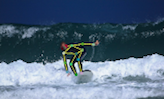
\includegraphics[width=5cm,height=4cm]{source/single.png}}
  \hspace{1in}
  \subfigure[Multi-person pose estimation]{
    \label{fig:subfig:b} %% label for second subfigure
    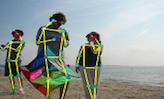
\includegraphics[width=5cm,height=4cm]{source/multi.png}}
  \caption{Figure 1: Human Pose Estimation. (a) is the example of single person pose estimation, only one person in a image. (b) is the example of multi-persion pose
  estimation. An image includes several peoples. We need to detect all the keypoints and group them into the right person ID.}
  \label{fig:1} %% label for entire figure
\end{figure}

\subsection{Single person Pose Estimation}
The works based on CNN usually adopts two methods: regress the coordinates of keypoints directly and regress the cofidence score map of keypoints. Toshev \textit{et al.} firstly introduce
CNN to solve pose estimation problem in the work of DeepPose\cite{toshev2014deeppose}, which proposes a cascade of CNN keypoint coordinate regressors to deal with pose estimation. Tompson \textit{et al.}\cite{tompson2014joint}
attempt to solve the problem by predicting heatmaps of keypoints using CNN and graphical models.
Using heatmap as the supervised label can provide more robust information, hence recently most of work focus on predicting heatmaps.
For example, latest works such as Wei \textit{et al.}\cite{wei2016convolutional} and Newell \textit{et al.}\cite{newell2016stacked} show great performance via generating the score map of keypoints using very
deep convolutional neural networks.

\subsection{Multi-person Pose estimation}
Multi-person pose estimation is gaining increasing popularity recently because of the high demand for the real-life applications.
However, multi-person pose estimation is challenging owing to occlusion, various gestures of individual persons and unpredictable interactions between different persons.
The approach of multi-person pose estimation is mainly divided into two categories: bottom-up approaches and top-down approaches.

\subsubsection{Bottom-Up Approaches}

Bottom-up approaches\cite{newell2017associative, insafutdinov2016deepercut, pishchulin2016deepcut} directly predict all keypoints at first and assemble them into full poses of all persons.
DeepCut\cite{pishchulin2016deepcut} interprets the problem of distinguishing different persons in an image as an Integer Linear Program (ILP) problem and partition
part detection candidates into person clusters.
Then the final pose estimation results are obtained when person clusters are combined with labeled body parts.
DeeperCut\cite{insafutdinov2016deepercut} improves DeepCut\cite{pishchulin2016deepcut} using deeper ResNet\cite{he2016deep} and employs image-conditioned pairwise terms to get better performance.
Zhe Cao \textit{et al.}\cite{cao2016realtime} map the relationship between keypoints into part affinity fields (PAFs) and assemble detected keypoints into different poses of people.
Newell \textit{et al.}\cite{newell2017associative} simultaneously produce score maps and pixel-wise embedding to group the candidate keypoints to different people to get final multi-person pose estimation.

\subsubsection{Top-down Approaches}
Top-down approaches\cite{huang2017coarse, papandreou2017towards, he2017mask} interpret the process of detecting keypoints as a twostage pipeline, that is, firstly locate and crop all persons from image,
and then solve the single person pose estimation problem in the cropped person patches.
Papandreou \textit{et al.}\cite{papandreou2017towards} predict both heatmaps and offsets of the points on the heatmaps to the ground truth location, and then uses the heatmaps with offsets to obtain the final predicted location of keypoints.
Mask-RCNN\cite{he2017mask} predicts human bounding boxes first and then crops the feature map of the corresponding human bounding box to predict human keypoints.
If top-down approach is utilized for multi-person pose estimation, a human detector as well as single person pose estimator is important in order to obtain a good performance.

\subsubsection{Human detection}
Human detection approaches are mainly guided by the RCNN family\cite{girshick2014rich, girshick2015fast, ren2015faster}, the upto-date detectors of which are\cite{lin2017feature, he2017mask}.
These detection approaches are composed of two-stage in general.
First generate boxes proposals based on default anchors, and then crop from the feature map and further refine the proposals to get the final boxes via R-CNN network.


\section{COCO dataset}

COCO\cite{lin2014microsoft} is a large-scale object detection, segmentation, and captioning dataset\footnote{More details about COCO dataset can be found in http://cocodataset.org/}.
For different tasks like object detection, keypoint detection, stuff segmentaion, etc, COCO dataset can be seperated as different sub-datasets.
Here we only introduce the human keypoint dataset.


\subsection{Dataset statistic}
The coco keypoint dataset was split up into 3 parts: train-set, validation-set, test-set.
And test-set is further divided into 2 parts: test-dev for evaluating the model in the usual time and test-challenge for evaluating the model during the competition.
It should be noted here that only labels of train-set and validation-set are available.
In order to extend the train-set, we extracted a small subset of the validation-set called mini-val for evaluating our model,
and the rest of validation-set and train-set merged into one larger train-set called train-val.

\captionsetup[table]{labelformat=empty}
\begin{table}[!hbp]
  \centering
  \begin{tabular}{|c|c|c|c|c|c|c|}
  \hline
            & train-set & validation-set & test-dev & test-challenge & train-val & mini-val \\
  \hline
  images numbers & 39935 & 19010 & 20000 & 20000 & 56599 & 2346\\
  \hline
  instances numbers & 105968 & 50197 & unknown & unknown & 149813 & 6352\\
  \hline
  keypoints numbers & 1161667  & 548831 & unknown & unknown & 1642283 & 68215\\
  \hline
  \end{tabular}
  \caption{Table 1: The statistics of datasets}
\end{table}

\subsection{Annotation format}

Each person(instance) annotations contains a series of fields. \textbf{1.} id: Indicates the global id of this instance. \textbf{2.} image\_id: Indicates which images this person belongs to. \textbf{3.} bbox: Indicates the location of this person in the image.
\textbf{4.} keypoints: A length 3*17 array, indicates the details of the keypoints. Each keypoint has a 0-indexed location x,y and a visibility flag v defined as v=0: not labeled (in which case x=y=0), v=1: labeled but not visible, and v=2: labeled and visible.
\textbf{5.} s: Indicates the square root of the object segment area.

There are 17 keypoints: 0: nose, 1: left eye, 2: right eye, 3: left ear, 4: right ear, 5: left shoulder, 6: right shoulder, 7: left elbow, 8: right elbow, 9: left wrist, 10: right wrist, 11: left hip, 12: right hip, 13: left knee, 14: right knee, 15: left ankle, 16: right ankle.

\begin{lstlisting}
annotation{
  "id" : int,
  "image_id" : int,
  "bbox" : [x, y, weight, height],
  // x, y is the coordinate of the top-left point of the bbox.
  "keypoints" : [x1, y1, v1, ...]
  "s" : float
}
\end{lstlisting}

\subsection{Metric}

The core idea behind evaluating keypoint detection is to mimic the evaluation metrics used for object detection, namely average precision (AP) and average recall (AR) and their variants.
At the heart of these metrics is a similarity measure between ground truth objects and predicted objects.
In the case of object detection, the IoU(Intersection over Union) serves as this similarity measure (for both boxes and segments).
Thesholding the IoU defines matches between the ground truth and predicted objects and allows computing precision-recall curves.
To adopt AP/AR for keypoints detection, we only need to define an analogous similarity measure.
Here an object keypoint similarity (OKS) which plays the same role as the IoU.

As mentioned before, for each object, ground truth keypoints have the form $[x_{1},y_{1},v_{1},...,x_{k},y_{k},v_{k}]$, where x,y are the keypoint locations and v is a visibility flag defined as v=0: not labeled, v=1: labeled but not visible, and v=2: labeled and visible.
Each ground truth object also has a scale s which is defined as the square root of the object segment area.

For each object, the keypoint detector must output keypoint locations and an object-level confidence.
Predicted keypoints for an object should have the same form as the ground truth: $[x_{1},y_{1},v_{1},...,x_{k},y_{k},v_{k}]$.
However, the detector's predicted $v_{i}$ are not currently used during evaluation, that is the keypoint detector is not required to predict per-keypoint visibilities or confidences.

The object keypoint similarity (OKS) is defined as:

\[ OKS =  \frac{\sum_{i}[exp(-d_{i}^{2} / 2s^{2}k_{i}^{2}) \delta (v_{i}>0)]}{\sum_{i} [\delta(v_{i}>0)]} ...................(1) \]

The $d_{i}$ are the Euclidean distances between each corresponding ground truth and detected keypoint and the $v_{i}$ are the visibility flags of the ground truth (the detector's predicted $v_{i}$ are not used).
To compute OKS, we pass the $d_{i}$ through an unnormalized Guassian with standard deviation $sk_{i}$, where s is the object scale and $k_{i}$ is a per-keypont constant that controls falloff.
For each keypoint this yields a keypoint similarity that ranges between 0 and 1.
These similarities are averaged over all labeled keypoints (keypoints for which $v_{i}>0$).
Predicted keypoints that are not labeled ($v_{i}=0$) do not affect the OKS.
Perfect predictions will have OKS=1 and predictions for which all keypoints are off by more than a few standard deviations sκi will have OKS~0.
The OKS is analogous to the IoU.
Given the OKS, we can compute AP and AR just as the IoU allows us to compute these metrics for box/segment detection.

The final metric for COCO keypoint dataset is shown as below:

\captionsetup[figure]{labelformat=empty}
\begin{figure}[htbp]
  \centering
  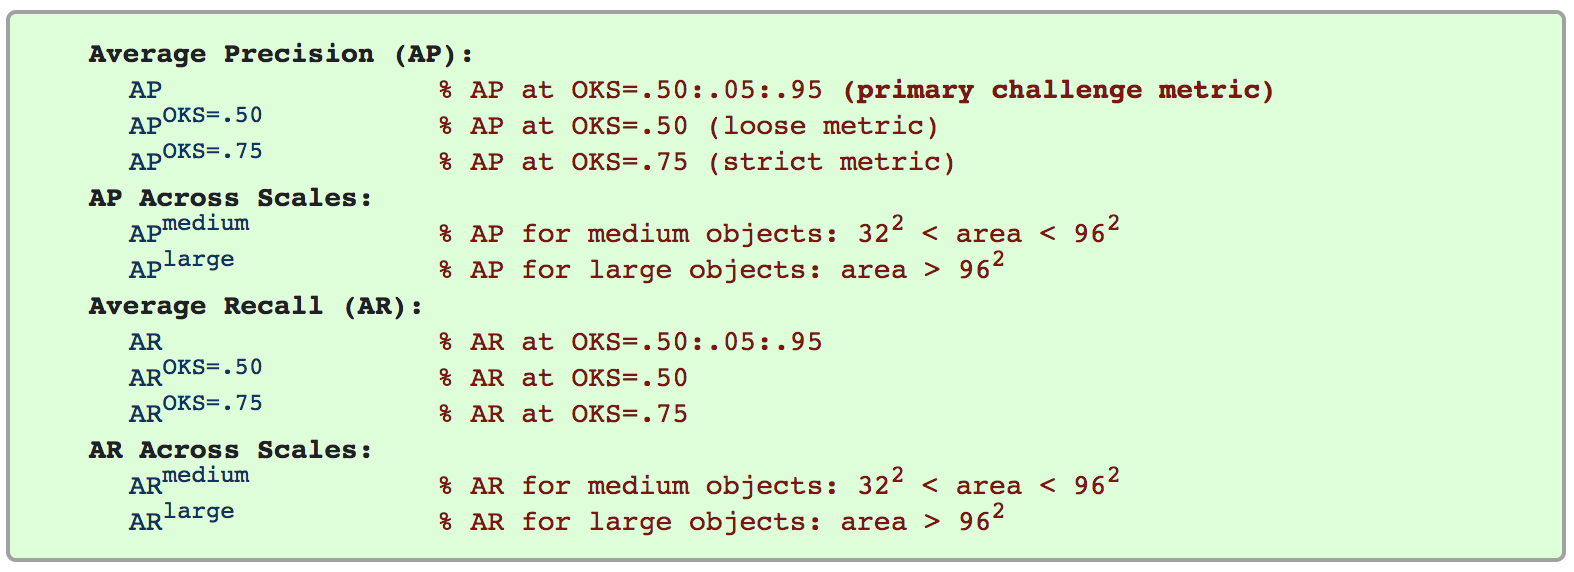
\includegraphics[width=16cm,height=6cm]{source/metric.png}
  \caption{Figure 2: The final metrics for COCO keypoint task. }
\end{figure}




%%% Local Variables:
%%% mode: latex
%%% TeX-master: "rapportM2R"
%%% End:


%% Copyright (C) 2008 Johan Oudinet <oudinet@lri.fr>
%%
%% Permission is granted to make and distribute verbatim copies of
%% this manual provided the copyright notice and this permission notice
%% are preserved on all copies.
%%
%% Permission is granted to process this file through TeX and print the
%% results, provided the printed document carries copying permission
%% notice identical to this one except for the removal of this paragraph
%% (this paragraph not being relevant to the printed manual).
%%
%% Permission is granted to copy and distribute modified versions of this
%% manual under the conditions for verbatim copying, provided that the
%% entire resulting derived work is distributed under the terms of a
%% permission notice identical to this one.
%%
%% Permission is granted to copy and distribute translations of this manual
%% into another language, under the above conditions for modified versions,
%% except that this permission notice may be stated in a translation
%% approved by the Free Software Foundation
%%
\chapter{Conclusion}
I was mainly responsible for the COCO 2018 keypoint competition during this internship.
The time-line is like below:
\begin{enumerate}
  \item April $\sim$ May: Get similar to Human Pose Estimation problem and review related works and codes.
  \item May $\sim$ June: Think that dataset is a choke point and more data is necessary. Try to generate train data using GAN\cite{goodfellow2014generative}.
  \item June $\sim$ Mid-July: Design a novel network.
  \item Mid-July $\sim$ Mid-August(Deadline of Competition): Try to ensemble and fine-tune hyper-parameters.
\end{enumerate}

Finally, we proposed a novel multi-stage network which can learn both normal poses and hard poses well.
Based on the proposed algorithm, we achieved state-of-art results on the COCO keypoint benchmark, with average
precision at $77.8\%$ mAp on the COCO test-dev dataset and $76.4\%$ on the COCO test-challenge dataset, which is a $4.8\%$ mAp
relative improvement compared with $73.0\%$ from the COCO 2017 keypoint challenge.

\textbf{Our team was invited to make a presentation in ECCV2018, September 8 - 14 in Munich, Germany}\footnote{More details about the conference can be found in https://eccv2018.org/}.

Here, I want to record some feeling about this competition experience.
There are two main points:
\begin{enumerate}
  \item \textbf{The hardest part is the beginning and ending period.} At the beginning, I was new to Human Pose Estimation problem totally.
  At that time, leader requested me to do a quick review of the recent related works and make a presentation.
  I read papers every day and studied the source codes, but improve myself rapidly.
  In the last few weeks, all the ideas have been tried and our results on COCO benchmark have been stalled.
  I remember clearly that I was particularly anxious every day during that time.
  \item \textbf{Preparing the competition is totally different from doing research work.}
  In my opinion, when doing research, we should believe that one idea is useful and stick to it.
  But when preparing the competition, we may try many ideas and each idea has a end time point in order to avoid risk.
  For example, throughout the whole May, I have tried using GAN to generate new train samples. However it didn't work finally.
  So we started another attempt even though we all thought generating train data is a meaningful work. 
\end{enumerate}


%%% Local Variables:
%%% mode: latex
%%% TeX-master: "rapportM2R"
%%% End:


\chapter*{Acknowledgement}
At last, i would like to point out that i couldn’t nish this internship
successfully without someones, and here i give my most sincere thanks to them.
Firstly, i will express thanks to Zhicheng WANG, one of my team leader. It’s him
that taught me the basic knowledge of DL, like CNN, Resnet, frameworks, etc. He
also explained papers to me clearly and carefully. In fact, he leads me into the domain
CV&DL.
Next, iwould like to thank for Gang YU, my another team leader. During August,
i did some research work about SOT(single object tracking), which is supervised by
him. He gave me lots of help, like correcting my wrong opinions and reviewing my
codes.
Finally but with same importance, my colleagues helped me a lot when i encountered
some problems about software or hardware, i will always appreciate that.

\bibliographystyle{plain}
\bibliography{rapport_m2_AIC}

\appendix

% \input{appendixA}

\end{document}


%%% Local Variables:
%%% mode: latex
%%% TeX-master: "rapportM2R"
%%% End:
